\documentclass{article}
\usepackage{graphicx}
\graphicspath{ {./images/} }

\title{UDA Experiments}
\author{Michael Morris}

\begin{document}
\maketitle

\section{Introduction}
Semi supervised learning is a method of training machine learning models which leverages unlabelled data. There are many ways of doing this, typically by using unlabelled samples to create a decision boundary.

\begin{figure}[h]
  \begin{center}
    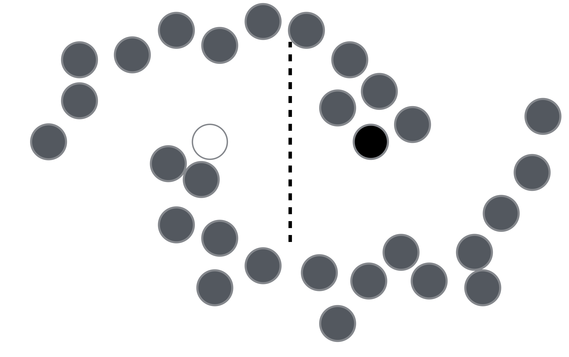
\includegraphics[width=.4\textwidth]{SSL}
    \caption{Decision boundary with unsupervised examples}
  \end{center}
\end{figure}

Its intuitive which class each unlabelled sample would be in, and can be mathematically found based on some assumptions:
\begin{itemize}
  \item Points which are close together are likely to be in the same class 
  \item The data tends to form distinct clusters
  \item The data can be expressed in much lower dimensions than its inputs.
\end{itemize}
This 








\end{document}